\documentclass[main.tex]{subfiles}
\begin{document}
\begin{bmcsex}{Pullout with bond damage-softening}{e33_pullout_frp_damage}
\noindent This example demonstrates the local nature of debonding
    with propagating damage process zone. Notice the constant 
    energy release rate.
 \\
\begin{center}
            
{\scriptsize 
\begin{longtable}{lrp{4cm}}\toprule
\textbf{\textsf{Model parameter}} 
& 
\textbf{\textsf{Symbol = Value [Unit]}} 
&
\textbf{\textsf{Description}}  \\\midrule \midrule
\texttt{u\_f0\_max} & $u_{\mathrm{f},0,{\max}}$ = 0.3 [mm] & {\footnotesize maximum displacement of the pulled reinforcement}  \\
            \texttt{tolerance} & None = 0.0001 [None] & {\footnotesize None}  \\
            \texttt{fixed\_boundary} & None = non-loaded end (matrix) [None] & {\footnotesize which side of the specimen is fixed}  \\
            \texttt{n\_e\_x} & $n_\mathrm{E}$ = 100 [-] & {\footnotesize number of finite elements along the embedded length}  \\
            \texttt{k\_max} & None = 500 [None] & {\footnotesize None}  \\
            \midrule
\multicolumn{3}{l}{\textbf{\textsf{Geometry: geometry}}}\\

\texttt{geometry.L\_x} & $L$ = 500.0 [$\mathrm{mm}$] & {\footnotesize embedded length}  \\
            \midrule
\multicolumn{3}{l}{\textbf{\textsf{CrossSection: cross\_section}}}\\

\texttt{cross\_section.A\_f} & $A_\mathrm{f}$ = 16.67 [$\mathrm{mm}^2$] & {\footnotesize reinforcement area}  \\
            \texttt{cross\_section.A\_m} & $A_\mathrm{m}$ = 1540.0 [$\mathrm{mm}^2$] & {\footnotesize matrix area}  \\
            \texttt{cross\_section.P\_b} & $P_\mathrm{b}$ = 1.0 [$\mathrm{mm}$] & {\footnotesize perimeter of the bond interface}  \\
            \midrule
\multicolumn{3}{l}{\textbf{\textsf{MATSBondSlipFRPDamage: mats\_eval}}}\\

\texttt{mats\_eval.omega\_fn\_type} & None = FRP [None] & {\footnotesize None}  \\
            \texttt{mats\_eval.E\_f} & None = 200000.0 [None] & {\footnotesize None}  \\
            \texttt{mats\_eval.E\_m} & None = 30000.0 [None] & {\footnotesize None}  \\
            \midrule
\multicolumn{3}{l}{\textbf{\textsf{FRPDamageFn: omega\_fn}}}\\

\texttt{mats\_eval.omega\_fn.s\_0} & $s_0$ = 0.00917278625472 [None] & {\footnotesize elastic strain limit}  \\
            \texttt{mats\_eval.omega\_fn.b} & $b$ = 10.4 [None] & {\footnotesize parameter controls the damage function}  \\
            \texttt{mats\_eval.omega\_fn.Gf} & $G_\mathrm{f}$ = 1.19 [None] & {\footnotesize fracture energy}  \\
            
\multicolumn{3}{r}{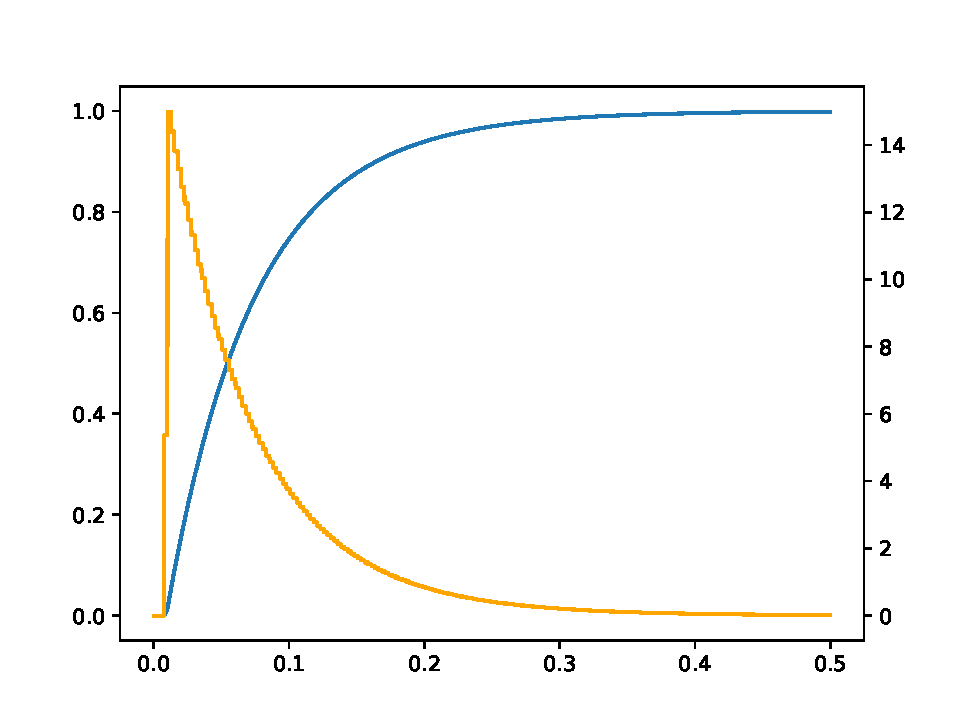
\includegraphics[width=5cm]{examples/e33_pullout_frp_damage/fig_FRP_damage_function.pdf}}\\
\bottomrule 
\end{longtable}
}

    Loading is applied at the right end of the specimen. The specimen
    is fixed at the unloaded end by prescribing zero matrix displacement. 
    Four stages of loading are displayed as marked in the
    loading scenario and in the pull-out curve.
    \begin{longtable}{c}
\mbox{
    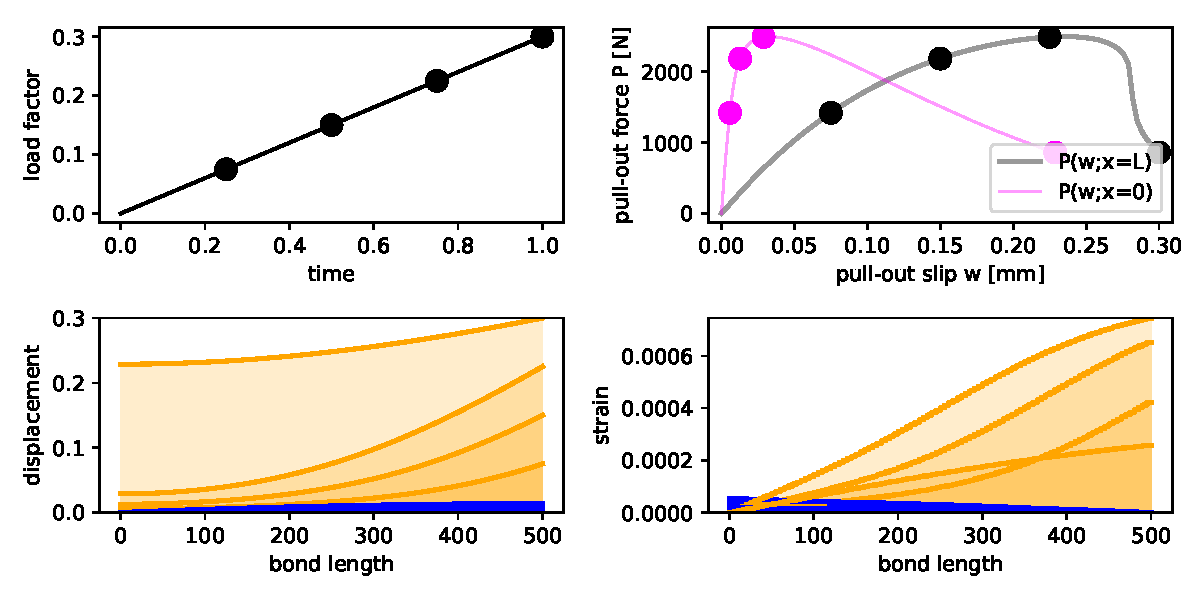
\includegraphics[width=0.8\textwidth]{examples/e33_pullout_frp_damage/fig_frictional_bond01.pdf}
    }\\
    
    \mbox{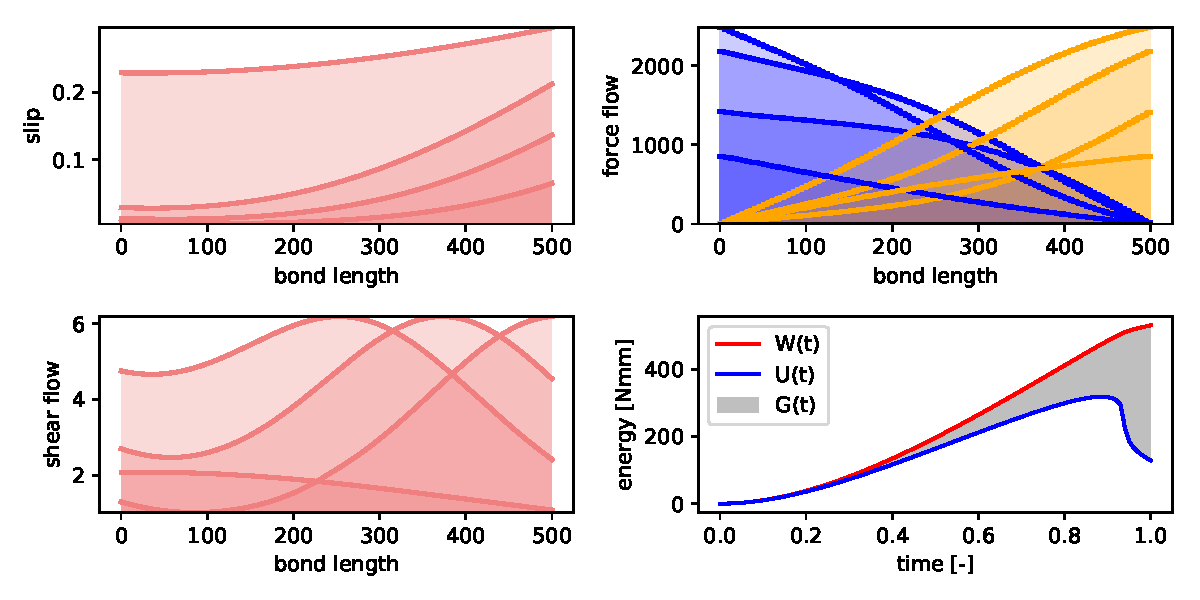
\includegraphics[width=0.8\textwidth]{examples/e33_pullout_frp_damage/fig_frictional_bond02.pdf}}

    
    \end{longtable}
    \end{center}
            \end{bmcsex}
\end{document}
    